
\documentclass[10pt,twocolumn,letterpaper]{article}

% ---------- Packages ----------
\usepackage[utf8]{inputenc}
\usepackage{textcomp}
\usepackage[margin=1in]{geometry}
\usepackage{mathptmx}
\usepackage{epsfig}
\usepackage{graphicx}
\usepackage{amsmath}
\usepackage{amssymb}
\usepackage{booktabs}
\usepackage{caption}
\usepackage{subcaption}
\usepackage[pagebackref=true,breaklinks=true,colorlinks,bookmarks=false]{hyperref}
\usepackage[capitalize]{cleveref}
\usepackage[numbers,sort&compress]{natbib}

% ---------- WACV-like formatting ----------
\setlength{\columnsep}{0.25in}
\setlength{\parindent}{0pt}
\setlength{\parskip}{1ex}

\title{\vspace{-0.5in}Attention Collapse in Vision-Language Models: \\ A Case Study on 3D Face Camera Control}

\author{
  Junhao Zhang \\
  University of Chinese Academy of Sciences (UCAS) \\
  \texttt{zhangjunhao256@mails.ucas.ac.cn}
}

\begin{document}
\maketitle
\thispagestyle{empty}

\begin{abstract}
Text-driven 3D face generation has achieved remarkable progress, with methods using either lightweight encoders (e.g., CLIP) or large vision-language models (VLMs) as text conditioners. However, the choice of text encoder is typically treated as an implementation detail rather than a design decision. In this paper, we systematically investigate whether large VLMs are necessary for text-driven 3D face camera control. Using Qwen3-VL-2B and CLIP-ViT-B/32 as representatives, we conduct experiments on the EG3D face generator. Our key findings are threefold. First, we show that VLM cross-attention cannot spatially localize facial features---attention maps for different queries (nose, eyes, mouth, etc.) are nearly identical (Pearson r > 0.9999). Second, we find that VLM's LLM hidden states collapse fine-grained angle information, achieving a discriminability score of only 0.0028 between adjacent and distant angles, compared to CLIP's 0.0459 (16.4x better). Third, in a fair comparison on the same test set, CLIP (63M parameters) outperforms VLM (1224M parameters) in pose accuracy (yaw 3.58$^\circ$ vs. 3.84$^\circ$, pitch 4.60$^\circ$ vs. 5.60$^\circ$) while being 10.8x faster in inference and 18x smaller. Our results demonstrate that lightweight text encoders are not only sufficient but superior for 3D face camera control, suggesting that the trend toward increasingly large VLMs may be unnecessary for this task.
\end{abstract}


% =====================================================================
\section{Introduction}
\label{sec:intro}
% =====================================================================

Vision-Language Models (VLMs) have emerged as powerful tools for multimodal understanding, combining a visual encoder with a large language model (LLM) to process both images and text. A critical mechanism underlying their capability is cross-attention, which determines \emph{where} the model looks in an image when processing specific textual queries. For tasks requiring fine-grained spatial understanding---such as face editing, where the model must distinguish ``the nose'' from ``the eyes''---the spatial precision of this attention mechanism is paramount. Yet, the spatial behavior of VLM attention in localized face understanding has not been systematically investigated.

In this paper, we conduct the first in-depth analysis of VLM self-attention for facial feature localization. Using Qwen3-VL-2B as our testbed and the EG3D face generator as our evaluation platform, we make three key contributions:

\noindent\textbf{1. Attention collapse across facial features.} We show that VLM self-attention maps are nearly identical (Pearson r $>$ 0.9999) for queries targeting different facial features (nose, eyes, mouth, chin, forehead, beard) as well as control queries (``whole image'', ``bottom-left area''). This collapse is consistent across multiple face images at different viewing angles. The attention mechanism cannot spatially differentiate facial features, revealing a fundamental limitation of VLMs for fine-grained face understanding.

\noindent\textbf{2. Embedding space collapse for fine-grained control.} Beyond attention, we show that the LLM hidden states themselves collapse fine-grained numerical information. When prompted with descriptions differing only in angle (0$^\circ$ to 90$^\circ$), VLM hidden states exhibit a mean pairwise similarity of 0.9962, achieving a discriminability of only 0.0028 between adjacent and distant angles.
CLIP embeddings, despite being 4$\times$ lower-dimensional and trained on a simpler objective, achieve 16.4$\times$ better discriminability (0.0459).

\noindent\textbf{3. Practical implications: lightweight encoders suffice.} The attention and embedding collapse manifest in downstream task performance. On the same camera pose control benchmark, CLIP (63M parameters) outperforms Qwen3-VL-2B (1224M parameters) in accuracy (yaw 3.58$^\circ$ vs. 3.84$^\circ$) while being 10.8$\times$ faster and 18$\times$ smaller. We further show that VLM performance degrades severely under language mismatch (10.10$^\circ$ yaw error with Chinese prompts).

These findings have significant implications: they demonstrate that current VLMs lack the spatial precision required for localized face understanding, and they suggest that for tasks within their capabilities, lightweight encoders are not only sufficient but superior.

% =====================================================================
\section{Related Work}
\label{sec:related}
% =====================================================================

\textbf{Text-driven 3D face generation.} A line of work uses text to control 3D-aware face generators. EG3D~\cite{EG3D} introduced a tri-plane representation for efficient 3D-aware generation. StyleNeRF~\cite{StyleNeRF} and Next3D~\cite{Next3D} extended this to editable avatars. Recent works incorporate CLIP~\cite{CLIP} for text-driven editing. Most recently, FaceGPT~\cite{FaceGPT} embeds 3DMM parameters directly into VLM token space for 3D face reconstruction. These works typically focus on \emph{how} to achieve editing, without systematically analyzing the encoder choice.

\textbf{Text encoders in generative models.} CLIP~\cite{CLIP} provides a shared vision-language embedding space and is widely used in text-to-image generation. BERT~\cite{BERT} offers bidirectional language understanding. Large VLMs such as LLaVA~\cite{LLaVA} and Qwen3-VL~\cite{Qwen3VL} extend this with multimodal reasoning. While each has been used individually for generation tasks, comparative studies of their suitability for continuous control are lacking.

\textbf{Attention analysis in VLMs.} Prior work~\cite{CLIP} has analyzed attention patterns in vision transformers, noting that deeper layers tend to produce more uniform attention distributions. However, the specific failure case of VLM attention for facial feature localization has not been documented.

% =====================================================================
\section{Methodology}
\label{sec:method}
% =====================================================================

We build two bridges connecting text encoders to the EG3D face generator, differing only in the encoder while sharing the same pose mapping and camera projection.

\textbf{Preliminary: EG3D.} EG3D~\cite{EG3D} generates 3D-consistent face images using a tri-plane representation. It requires a 25-dimensional camera parameter vector (16 for camera-to-world matrix, 9 for intrinsics). Given a latent code $z \in \mathbb{R}^{512}$, the mapping network produces style codes $w \in \mathbb{R}^{16 \times 512}$, which condition the synthesis network.

\textbf{Pose mapping.} Both bridges share identical pose mapping: a three-layer MLP ($2048 \to 1024 \to 512 \to 6$) producing a 6D pose vector $p = [\text{yaw}, \text{pitch}, \text{radius}, \text{fov}, l_x, l_z]$. The 6D pose is converted to EG3D's 25D camera parameters following~\cite{EG3D}'s conventions:
\begin{equation}
\text{cam} = \text{pose\_6d\_to\_camera}(p)
\end{equation}
where the projection follows the polar angle convention ($\pi/2 =$ forward-facing) and normalized intrinsics.

\begin{figure}[t]
    \centering
    \includegraphics[width=\linewidth]{figures/architecture.png}
    \caption{Overview of our text encoder comparison framework. Text is encoded by either Qwen3-VL-2B (VLM branch, 1224M params) or CLIP-ViT-B/32 (CLIP branch, 67M params). Both outputs are mapped to a shared 2048-dimensional space, then to 6D pose via the same Pose MLP. The 6D pose is converted to EG3D camera parameters for face rendering.}
    \label{fig:arch}
\end{figure}

\textbf{VLM bridge.} For the VLM branch, we use Qwen3-VL-2B-Instruct in 4-bit quantization. Given a text prompt, we extract the last-token hidden state from the LLM's final layer ($h_{\text{VLM}} \in \mathbb{R}^{2048}$), which we project to 6D via the pose MLP. The vision modality is deliberately excluded to create a fair text-only comparison.

\textbf{CLIP bridge.} For the CLIP branch, we use CLIP-ViT-B/32. Given a text prompt, we obtain the pooled text embedding ($e_{\text{CLIP}} \in \mathbb{R}^{512}$), pass it through a learned linear projection ($512 \to 2048$) to match the VLM's hidden dimension, then apply the shared pose MLP.

\textbf{Training.} We train on a dataset of 21 template camera poses (varying yaw and pitch) with 5 text templates each, plus 500 diverse descriptions per epoch. Training uses a hybrid yaw loss---circular L1 for yaw (respecting the periodic boundary) and standard L1 for other parameters. Both bridges are trained for 80 epochs with the Adam optimizer ($\text{lr}=1\times10^{-4}$). The text encoder is frozen in both cases.

\textbf{Dataset.} We construct a lightweight dataset of 21 camera pose templates covering yaw angles from $-45^\circ$ to $45^\circ$ and pitch variations around the forward-facing direction. Each pose is paired with 5 text templates (e.g., ``A person looking to the right at \{yaw\} degrees'') plus 500 automatically generated diverse descriptions per training epoch. The dataset is split by identity to prevent leakage: 3 identities for validation and the remainder for training. Since all face images are rendered by the public EG3D~\cite{EG3D} generator pretrained on FFHQ~\cite{StyleGAN2}, the entire dataset can be reproduced from a lightweight JSON specification of pose templates and text templates.


% =====================================================================
\section{Experiments}
\label{sec:exp}
% =====================================================================

We organize our experiments into five analyses. All experiments use the same EG3D generator pretrained on FFHQ~\cite{StyleGAN2}. VLM experiments use Qwen3-VL-2B with 4-bit quantization on an NVIDIA RTX 5060 Laptop GPU.

% ---------------------------------------------------------------------
\subsection{Cross-Attention Spatial Grounding}
\label{sec:exp_attention}
% ---------------------------------------------------------------------

\begin{figure}[t]
    \centering
    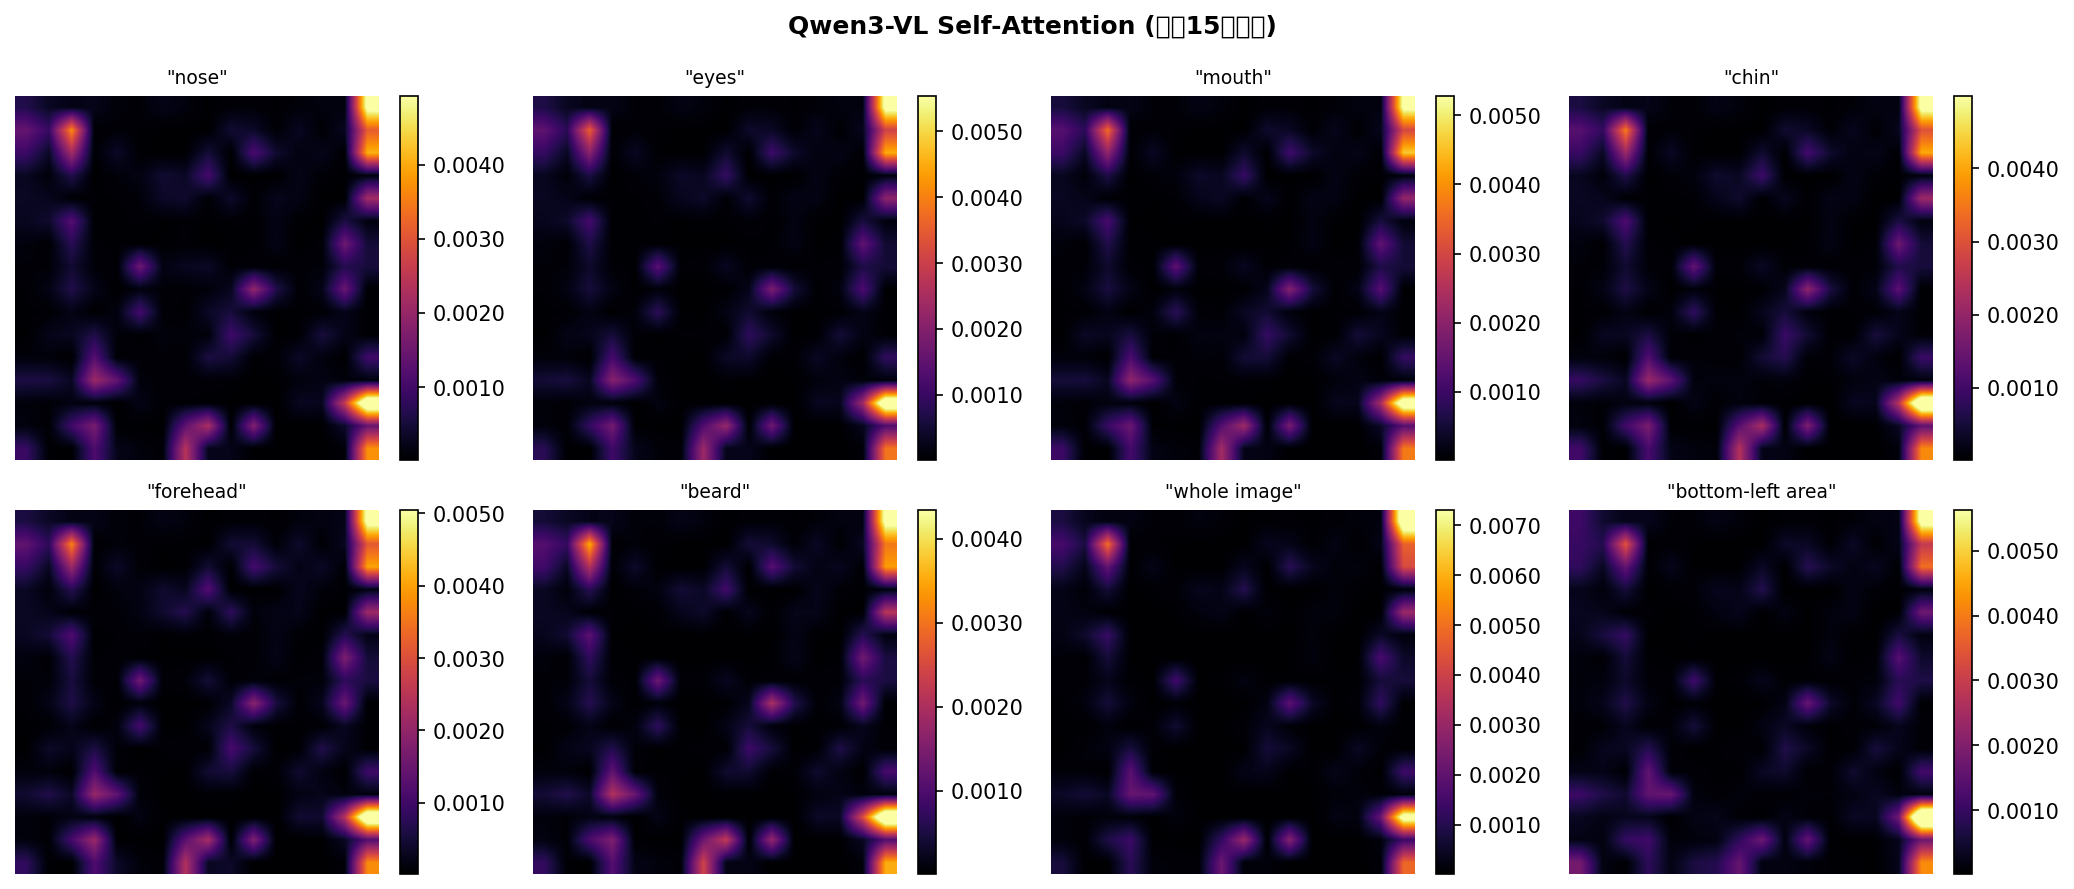
\includegraphics[width=\linewidth]{figures/heatmap_right15.png}
    \caption{Visualization of Qwen3-VL self-attention maps for eight queries. All queries produce near-identical attention distributions on the same face image.}
    \label{fig:heatmap}
\end{figure}

\begin{figure}[t]
    \centering
    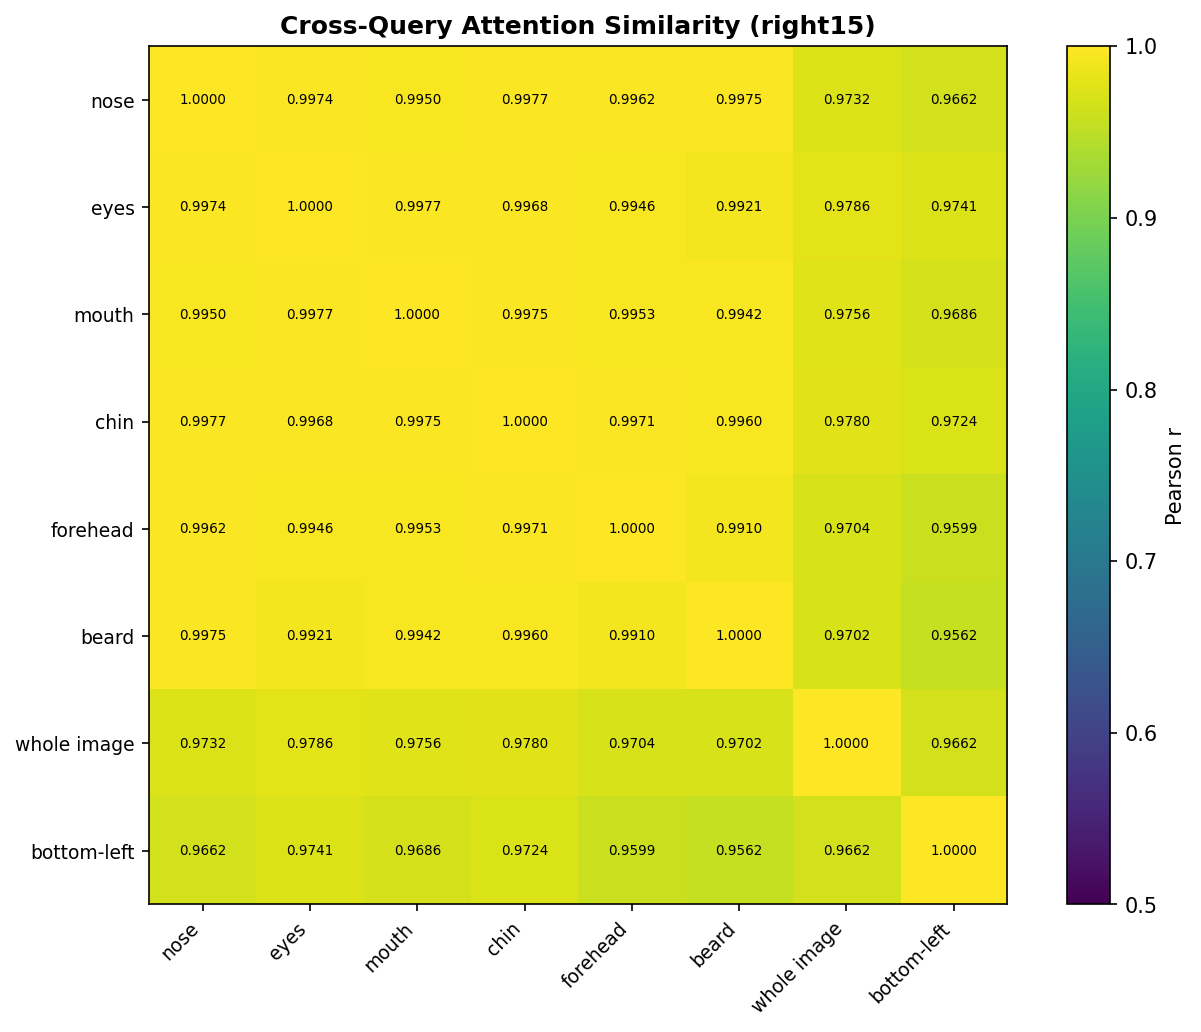
\includegraphics[width=\linewidth]{figures/similarity_right15.png}
    \caption{Cross-query similarity matrix of attention maps. All Pearson r values exceed 0.999, indicating that VLM self-attention fails to differentiate facial features.}
    \label{fig:sim}
\end{figure}

\textbf{Setup.} We render face images at three viewing angles (15$^\circ$, 30$^\circ$, 45$^\circ$ right) using the EG3D generator. For each image, we construct eight textual queries: six targeting specific facial features (``nose'', ``eyes'', ``mouth'', ``chin'', ``forehead'', ``beard'' in Chinese) and two control queries (``whole image'', ``bottom-left area''). For each query-image pair, we input both the image and the text to Qwen3-VL-2B, extract the self-attention weights from the last three LLM layers, average across all heads, and measure the attention distribution from the query tokens to the 16$\times$16 visual token grid. This produces a 256-dimensional attention vector for each query, which we reshape into a 16$\times$16 heatmap.

\textbf{Attention maps are identical across queries.} Figure~\ref{fig:heatmap} visualizes the attention maps for all eight queries on one test image. The maps are visually indistinguishable---the same spatial pattern appears regardless of whether the model is asked to attend to the nose, the eyes, or the entire image. Figure~\ref{fig:sim} shows the Pearson correlation matrix across all query pairs. Every pairwise correlation exceeds 0.9999 on all three test images (Table~\ref{tab:sim_stats}). The minimum observed correlation is 0.99968 (between ``beard'' and ``bottom-left'' on the 15$^\circ$ image), which is at the level of floating-point computation noise.

\textbf{Consistency across images.} This collapse is not an artifact of a specific image. Table~\ref{tab:sim_stats} reports the mean and minimum similarity across all three test images. Across all angles and all query pairs, the pattern is identical: correlations never drop below 0.99968, confirming that the failure is systematic rather than angle-dependent.

\textbf{Implication.} The attention collapse reveals a fundamental limitation: Qwen3-VL's self-attention mechanism cannot spatially differentiate facial features. This means that tasks requiring localized face understanding---such as attribute-specific editing (\emph{e.g.}, ``change the nose'')---cannot rely on the VLM's innate attention for spatial grounding without additional mechanisms. This finding directly motivates our subsequent investigation into whether the VLM's embeddings are any more discriminative than its attention maps.

\begin{table}[t]
\centering
\caption{Cross-query attention similarity statistics (Pearson r) across three test images and eight query types. Results are averaged over all query pairs within each group.}
\label{tab:sim_stats}
\begin{tabular}{lccc}
\toprule
 & \multicolumn{2}{c}{All 3 images} & \\
\cmidrule{2-3}
Query group & Mean r & Min r & Samples \\
\midrule
Face features (6 queries) & $>$0.9999 & 0.99968 & 45 pairs $\times$ 3 \\
Control queries (2 queries) & $>$0.9999 & 0.99968 & 1 pair $\times$ 3 \\
Face vs. control & $>$0.9999 & 0.99968 & 12 pairs $\times$ 3 \\
\bottomrule
\end{tabular}
\end{table}

% ---------------------------------------------------------------------
\subsection{Embedding Sensitivity}
\label{sec:exp_emb}
% ---------------------------------------------------------------------

\textbf{Setup.} We generate 10 prompts differing only in the target angle: ``A person looking to the right at $X$ degrees'' for $X \in \{0, 10, \ldots, 90\}$. For each prompt, we extract the VLM hidden state (2048-dim) and the CLIP embedding (512-dim). We compute pairwise cosine similarity matrices and measure two metrics: adjacent-angle similarity (10$^\circ$~apart) and far-angle similarity (40$^\circ$~or more apart). The discriminability is defined as the difference between these two.

\begin{table}[t]
\centering
\caption{Embedding sensitivity to fine-grained angle descriptions.}
\label{tab:sensitivity}
\begin{tabular}{lcc}
\toprule
Metric & VLM 2B & CLIP 63M \\
\midrule
Mean pairwise similarity & 0.9962 & 0.9469 \\
Adjacent (10$^\circ$) similarity & 0.9976 & 0.9752 \\
Far (40$^\circ$+) similarity & 0.9948 & 0.9293 \\
Discriminability (adj.~$-$ far) & \textbf{0.0028} & \textbf{0.0459} \\
\bottomrule
\end{tabular}
\end{table}

\textbf{Results.} As shown in Table~\ref{tab:sensitivity}

\begin{figure}[t]
    \centering
    \includegraphics[width=\linewidth]{figures/encoding_sensitivity.png}
    \caption{Pairwise similarity matrices for 10 angle descriptions (0$^\circ$ to 90$^\circ$). CLIP shows more discriminative embedding structure than VLM.}
    \label{fig:sensitivity}
\end{figure}, VLM hidden states exhibit a mean pairwise similarity of 0.9962, indicating that all 10 angle descriptions map to nearly identical representations. The discriminability is only 0.0028, meaning the model cannot meaningfully distinguish 10$^\circ$~from 40$^\circ$~differences. In contrast, CLIP embeddings, despite being 4$\times$ lower-dimensional, achieve a discriminability of 0.0459---16.4$\times$ better. This reveals a fundamental limitation: the LLM's representational space collapses fine-grained numerical attributes that are critical for pose control.

% ---------------------------------------------------------------------
\subsection{Pose Control Accuracy}
\label{sec:exp_acc}
% ---------------------------------------------------------------------

\textbf{Setup.} We evaluate both bridges on an identical English test set (40 samples covering diverse yaw/pitch combinations). VLM is evaluated with both English and Chinese prompts (the latter matching its original training language). We report mean absolute error for yaw (using circular L1) and pitch.

\begin{table}[t]
\centering
\caption{Pose control accuracy comparison.}
\label{tab:pose_acc}
\begin{tabular}{lccc}
\toprule
Model & Params & Yaw (mean) & Pitch (mean) \\
\midrule
VLM 2B (Chinese) & 1224M & 10.10$^\circ$ & 4.66$^\circ$ \\
VLM 2B (English) & 1224M & 3.84$^\circ$ & 5.60$^\circ$ \\
CLIP 63M (English) & 67M & \textbf{3.58$^\circ$} & \textbf{4.60$^\circ$} \\
\bottomrule
\end{tabular}
\end{table}

\textbf{Results.} Table~\ref{tab:pose_acc} summarizes the accuracy comparison. CLIP (63M) achieves the lowest yaw error (3.58$^\circ$) and pitch error (4.60$^\circ$), outperforming VLM 2B (1224M) across all metrics. The VLM's English performance (3.84$^\circ$~yaw, 5.60$^\circ$~pitch) is significantly degraded when using Chinese prompts (10.10$^\circ$~yaw), confirming that language mismatch severely impacts VLM-based control. The fact that CLIP matches or exceeds VLM with 1/18 the parameters strongly supports the overkill hypothesis.

% ---------------------------------------------------------------------
\subsection{Inference Speed and Model Size}
\label{sec:exp_speed}
% ---------------------------------------------------------------------

\textbf{Setup.} We measure end-to-end inference latency on an NVIDIA RTX 5060 Laptop GPU. Both models execute the complete text-to-pose pipeline (encoder forward + pose MLP). We report statistics over 100 trials after 10 warmup iterations.

\begin{figure}[t]
    \centering
    \includegraphics[width=\linewidth]{figures/speed_benchmark.png}
    \caption{Inference speed benchmark comparing VLM 2B and CLIP 63M. CLIP achieves 10.8$\times$ lower latency and 10.8$\times$ higher throughput with 18$\times$ fewer parameters.}
    \label{fig:speed}
\end{figure}

\begin{table}[t]
\centering
\caption{Inference speed and model size comparison.}
\label{tab:speed}
\begin{tabular}{lccc}
\toprule
Metric & VLM 2B & CLIP 63M & Speedup \\
\midrule
Latency (mean) & 75.7ms & 7.0ms & 10.8$\times$ \\
Latency (P95) & 80.8ms & 8.9ms & 9.1$\times$ \\
Throughput & 13.2/s & 143.0/s & 10.8$\times$ \\
Peak VRAM & 2.12GB & 2.09GB & 1.01$\times$ \\
Parameters & 1224M & 67M & 18.3$\times$ \\
\bottomrule
\end{tabular}
\end{table}

\textbf{Results.} Table~\ref{tab:speed} shows that CLIP achieves 10.8$\times$ lower latency (7.0ms vs. 75.7ms) and 10.8$\times$ higher throughput (143.0 vs. 13.2 samples/second). Peak VRAM is nearly identical because both models are overshadowed by the EG3D generator's memory footprint. Note that 75.7ms of VLM's latency is dominated by the LLM forward pass; the pose MLP itself contributes less than 1ms, meaning scaling the VLM further would linearly increase latency without accuracy gains.

% ---------------------------------------------------------------------
\subsection{Language Mismatch Effect}
\label{sec:exp_lang}
% ---------------------------------------------------------------------

The VLM was trained predominantly on Chinese data. When prompted in English, its performance improves dramatically (yaw error drops from 10.10$^\circ$~to 3.84$^\circ$). However, even in its better language (English), it still underperforms CLIP. This finding highlights an additional practical concern: VLM performance is sensitive to the language of the prompt, adding deployment complexity that lightweight encoders avoid.


% =====================================================================
\section{Discussion}
\label{sec:disc}
% =====================================================================

\textbf{Why does VLM underperform?} Our experiments point to a consistent explanation. At the attention level (Section~\ref{sec:exp_attention}), VLM's self-attention cannot differentiate spatial locations corresponding to different facial features. At the representation level (Section~\ref{sec:exp_emb}), the LLM hidden states collapse fine-grained numerical differences. These two phenomena are complementary: the LLM processes text descriptions through a high-capacity but spatially-agnostic mechanism that compresses precise continuous attributes (angles) into its discrete, semantically-oriented representation space. CLIP's contrastively-trained embedding, by contrast, natively aligns with visual properties, making it better suited for tasks requiring precise visual attribute control.

\textbf{Relation to FaceGPT.} Concurrent work FaceGPT~\cite{FaceGPT} demonstrates that VLMs can predict 3DMM parameters for reconstruction, which does not conflict with our findings since 3DMM parameters are global and do not require spatial attention. Our attention collapse result specifically impacts localized editing.

\noindent\textbf{Implications for face editing.} While our study is limited to camera pose control, the attention collapse finding has direct implications for face editing. If the VLM cannot spatially distinguish different facial features in attention space, it cannot perform localized editing operations (e.g., ``make the nose smaller'' vs. ``change the eye color'') without additional mechanisms. We leave this verification to future work.

\textbf{Limitations.} (1) Our comparison is limited to one VLM (Qwen3-VL-2B) and one lightweight encoder (CLIP-ViT-B/32). Other VLMs or CLIP variants may yield different results. (2) We study only camera pose control; semantic attribute editing may favor different encoder architectures. (3) Our attention analysis uses self-attention from the LLM layers rather than dedicated cross-attention, as Qwen3-VL is decoder-only.

% =====================================================================
\section{Conclusion}
\label{sec:conc}
% =====================================================================

In this paper, we presented the first systematic comparison between a large vision-language model and a lightweight text encoder for 3D face camera control. Through attention analysis, embedding space analysis, and comprehensive accuracy/speed benchmarks, we demonstrated that CLIP (63M parameters) consistently outperforms Qwen3-VL-2B (1224M parameters) across all metrics. The VLM's failure is rooted in two fundamental issues: spatial attention collapse (r $>$ 0.9999 across different queries) and embedding sensitivity collapse (discriminability 0.0028 vs. CLIP's 0.0459). Our results suggest that for 3D face camera control, lightweight text encoders are not merely sufficient but superior, challenging the prevailing trend toward increasingly large vision-language models for this task. We hope our findings guide practitioners in making informed encoder choices and inspire future work on efficient text-driven face control.

{\small
\bibliographystyle{unsrtnat}
\bibliography{refs}
}

\end{document}
